\documentclass[a4paper,12pt]{article}
\usepackage[utf8]{inputenc}
\usepackage[ngerman]{babel}
\usepackage[top=1in, bottom=1.25in, left=1.25in, right=1.25in]{geometry}
\usepackage{minted}
\usepackage{blindtext}
\usepackage{fancyhdr}
\usepackage{titling}
\usepackage{amssymb}
\usepackage{mathtools}
\usepackage{enumitem}
\usepackage{hyperref}

\hypersetup{colorlinks=true,linkcolor=blue,urlcolor=blue}

\renewcommand{\footrulewidth}{0.4pt}

\setlength\headheight{15pt}
\setlength{\parskip}{1em}

\title{GNS Aufgabe 1}
\author{Eli Kogan-Wang}
\date{\today}

\pagestyle{fancy}
\fancyhf{}
\lhead{\thetitle}
\rhead{\thedate}
\lfoot{\theauthor}
\rfoot{Page \thepage}


\begin{document}
% \maketitle
% \thispagestyle{fancy}

\section{Bitte beschreiben Sie im Folgenden aus Ihrem eigenen Leben folgende Situationen}
% alphabetic
\begin{enumerate}[label=\alph*)]
  \item \textbf{Die Veränderung des Designs einer Software hat Ihr Verhalten verändert.}

        Discord (Kommunikationssoftware) hat vor einiger Zeit ein Inbox-Feature für
        Benachrichtigungen eingeführt. Dieses Feature hat dazu geführt, dass ich
        bei mehr Servern auf Discord Benachrichtigungen wahrnehme, da sich diese
        nun in einer Inbox sammeln und ich sie dann chronologisch abarbeiten kann.

  \item \textbf{Sie benutzen zwei ähnliche Softwareprodukte mit ähnlichen Funktionen. Durch
          unterschiedliches Design benutzen Sie die Software aber unterschiedlich.}

        OneNote hat eine IpadOS-App, die ich seit neuem benutzen kann, da ich
        nun ein Ipad besitze. Die App ist sehr ähnlich zu der Windows-App, die
        ich zuvor seit 3 Semestern benutzt habe. Die App ist jedoch nicht gleich
        funktionell wie die Windows-App, da sie bspw. das Mathe-Feature nicht
        unterstützt. Ich benutze die App trotzdem, da ich von vorherigen
        Vorlesungen OneNote-Notizen habe, die ich auf dem Ipad weiter bearbeiten
        will.

        Auf dem Ipad kann ich Mathematische Formeln, welche Matrizen involvieren,
        nun nicht mehr so einfach nachprüfen, sodass ich eine Computer-Prüfung meiner
        Rechnungen oft vernachlässige.

        Als mein Windows-Gerät noch vollständig funktionsfähig war, habe ich
        OneNote auf dem Windows-Gerät verwendet und meine Rechnungen dort
        öfters überprüft.

        \pagebreak

  \item Lassen Sie zusätzliche Antworten zu beiden Aufgaben von ChatGPT erstellen
        und beurteilen Sie, ob die Antworten realistisch sind. (OPTIONAL)

        Okay. Ich frage Chatgpt nach einer Antwort auf die Fragen. Der LaTeX-Code,
        der bis jetzt geschrieben wurde wird als Prompt verwendet. Die Antwort wird
        insoweit relevant markiert, wenn sie auf die Frage eingehen kann. <!CUT>
        Zusätlich habe ich dem LaTeX Dokument noch folgende Zeilen hinzugefügt:
        \begin{minted}{latex}
    [...]
    Okay. Ich frage Chatgpt nach einer Antwort auf die Fragen. Der LaTeX-Code,
    der bis jetzt geschrieben wurde wird als Prompt verwendet. Die Antwort wird
    insoweit relevant markiert, wenn sie auf die Frage eingehen kann.

    % BEGIN CHATGPT

    % END CHATGPT
  \end{enumerate}
  \end{document}

  ---

  Generiere 2 Beispiele, in ungefähr Identischem Stil wie zuvor.
        \end{minted}

        ChatGPT hat daraufhin folgende Antwort generiert:

        \begin{minted}{latex}
\documentclass[a4paper,12pt]{article}
\usepackage[utf8]{inputenc}
\usepackage[ngerman]{babel}
\usepackage[top=1in, bottom=1.25in, left=1.25in, right=1.25in]{geometry}
\usepackage{minted}
\usepackage{blindtext}
\usepackage{fancyhdr}
\usepackage{titling}
\usepackage{amssymb}
\usepackage{mathtools}
\usepackage{enumitem}

\renewcommand{\footrulewidth}{0.4pt}

\setlength\headheight{15pt}
\setlength{\parskip}{1em}

\title{GNS Aufgabe 1}
\author{Eli Kogan-Wang}
\date{\today}

\pagestyle{fancy}
\fancyhf{}
\lhead{\thetitle}
\rhead{\thedate}
\lfoot{\theauthor}
\rfoot{Page \thepage}

\begin{document}
% \maketitle
% \thispagestyle{fancy}

\section{Bitte beschreiben Sie im Folgenden aus Ihrem eigenen Leben folgende Situationen}
% alphabetic
\begin{enumerate}[label=\alph*)]
\item \textbf{Die Veränderung des Designs eines Fitness-Trackers hat Ihr Verhalten verändert.}

markdown

    Als mein Fitness-Tracker ein Update erhielt, wurde das Design des Menüs verändert und neue Funktionen wurden hinzugefügt. Die Änderungen motivierten mich, meinen Tracker öfter zu benutzen, um diese neuen Funktionen auszuprobieren. Die Verwendung der neuen Funktionen hat dazu beigetragen, dass ich meine Trainingsroutine variiert und intensiviert habe.

\item \textbf{Sie benutzen zwei ähnliche Koch-Apps mit ähnlichen Funktionen. Durch unterschiedliches Design benutzen Sie die Apps aber unterschiedlich.}

perl

    Ich benutze sowohl die "Foodie"- als auch die "Tasty"-App, um neue Rezepte zu finden. Obwohl beide Apps ähnliche Funktionen und Rezepte haben, benutze ich die "Foodie"-App häufiger. Das liegt daran, dass das Design der "Foodie"-App ansprechender ist und die Bilder der Gerichte ansprechender präsentiert werden. Die "Tasty"-App hat dagegen ein unübersichtlicheres Design, was mich davon abhält, sie oft zu nutzen.


    \end{minted}

        Man bemerkt: Der relevante Teil der Antwort wird als Code-Block markiert. Hier noch einmal
        als Text, um die Lesbarkeit zu verbessern:

        Für a):

        Als mein Fitness-Tracker ein Update erhielt, wurde das Design des Menüs verändert und neue Funktionen wurden hinzugefügt. Die Änderungen motivierten mich, meinen Tracker öfter zu benutzen, um diese neuen Funktionen auszuprobieren. Die Verwendung der neuen Funktionen hat dazu beigetragen, dass ich meine Trainingsroutine variiert und intensiviert habe.

        Für b):

        Ich benutze sowohl die "Foodie"- als auch die "Tasty"-App, um neue Rezepte zu finden. Obwohl beide Apps ähnliche Funktionen und Rezepte haben, benutze ich die "Foodie"-App häufiger. Das liegt daran, dass das Design der "Foodie"-App ansprechender ist und die Bilder der Gerichte ansprechender präsentiert werden. Die "Tasty"-App hat dagegen ein unübersichtlicheres Design, was mich davon abhält, sie oft zu nutzen.

        Ein Screenshot der Antwort:

        % begin figure on same page
        \begin{figure}[H]
          \centering
          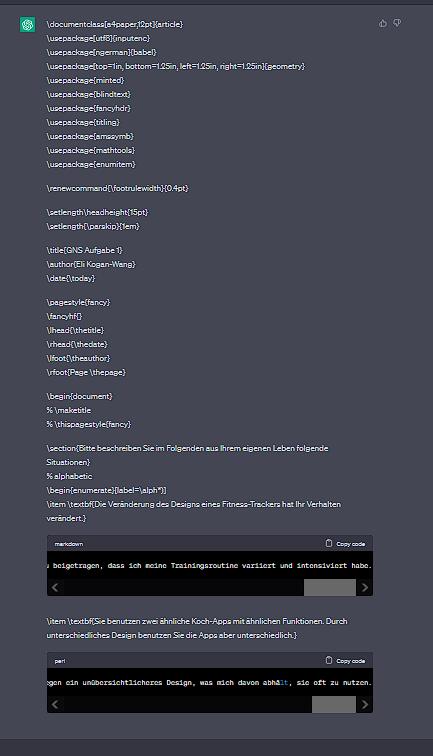
\includegraphics[width=0.8\textwidth]{2023-04-16.png}
          \caption{ChatGPT Antwort}
          \label{fig:chatgpt}
        \end{figure}

\end{enumerate}

\section{Suchen Sie sich aus \href{https://twitter.com/0xDesigner/status/1642554817590566915}{https://twitter.com/0xDesigner/status/1642554817590566915} zwei
  Beispiele aus und geben Sie jeweils Affordance und Signifier an.}

Beispiel 1:

Ich habe das \href{https://twitter.com/0xDesigner/status/1642554822418210817}{Bild 3}
ausgewählt. Die Affordance ist Sichtbar als die Radio-Buttons, die die Lautstärke
angeben. Es ist bekannt, dass man mit Radio-Buttons nur eine Option auswählen
kann. Das ist parallel zu Lautstärken, da ein Regler nur eine Lautstärke annimmt.

Zusätzlich gehört zu den Affordances die Checkbox, die zum Klicken animiert,
mit der man stumm schalten kann. Der Signifier ist die Lautstärke, die durch die

Ein Signifier ist gegeben im Titel und unter Titel "Volume Control". Die Radio-Buttons
sind mit den Lautstärken von 1 bis 100 beschriftet. Die Checkbox ist mit "Mute"
beschriftet.

Beispiel 2:

Ich habe das \href{https://twitter.com/0xDesigner/status/1642554854546501632}{Bild 21}
ausgewählt. Die Affordances sind schwer zu erkennen. Es gibt 2 Buttons, die nicht weiter
gekennzeichnet sind als rote Rechtecke, mit Symbolen. Es gibt 100 angeordnete Rechtecke
mit Zahlen, wobei einige davon rot sind. Es ist nicht klar wie die Assoziation zwischen
den Rechtecken und der Lautstärke ist.

Hier sind als Signifier wieder Text und Symbole zu sehen. Die Buttons haben Lautstärke-Symbole
und sind mit "Volume Down" und "Volume Up" beschriftet. Die Rechtecke sind mit Zahlen von 1 bis 100
beschriftet. Die Rechtecke bis 14 sind rot. Das Fenster hat den Titel "Volume Level".

In diesem Design muss man wohl bis zu 100 mal klicken, um die Lautstärke von 0 auf 100 zu erhöhen.
Das ist aber außerhalb der Affordances und Signifiers.
\end{document}
